\section{Obtained Results}

This section presents the compilation results, simulation behavior, and test scenarios executed on the dual-sensor temperature monitoring system with signal conditioning. The results demonstrate that the implemented three-stage conditioning pipeline (saturation, median filter, EWMA) correctly processes raw sensor readings before feeding them to the threshold alert FSM, producing stable and noise-resilient temperature monitoring.

\subsection{Build Process and Compilation}

The project was compiled using PlatformIO for the Arduino Mega 2560 target platform. The build process includes compilation of all lab-specific source files, the four reusable libraries (AnalogTempSensor, DigitalTempSensor, SignalConditioner, ThresholdAlert), and three libraries reused from previous labs (LcdDisplay, Led, StdioSerial), along with the external dependencies (FreeRTOS, OneWire, DallasTemperature, LiquidCrystal\_I2C).

\begin{figure}[H]
\centering
\IfFileExists{resources/ObtainedResults/build_results.png}{%
    
\includegraphics[width=0.85\textwidth]{resources/ObtainedResults/build_results.png}%
}{%
    \fbox{\parbox{0.83\textwidth}{\centering\color{gray}\small
        [Screenshot pending --- run \texttt{pio run -e lab3\_2} and\\
        capture the terminal output showing \texttt{[SUCCESS]}\\
        Save to resources/ObtainedResults/build\_results.png]}}%
}
\caption{PlatformIO build output for Lab 3.2 environment}
\label{fig:build_results}
\end{figure}

The build completed successfully with the following resource utilization:
\begin{itemize}
    \item \textbf{Flash memory}: The firmware size includes the FreeRTOS kernel, the DallasTemperature and OneWire libraries, the LiquidCrystal\_I2C library, and the new SignalConditioner module. The addition of the median filter circular buffer, insertion sort, and EWMA computation adds modest code overhead compared to Lab 3.1.
    \item \textbf{RAM}: 2\,431 bytes (29.7\% of 8\,192 bytes available). The increased RAM consumption relative to Lab 3.1 is attributable to the two SignalConditioner instances, each maintaining a circular buffer of up to 9 float values for the median filter window plus EWMA state variables. Despite this increase, the system retains comfortable headroom on the ATmega2560's 8 KB SRAM.
\end{itemize}

The modular architecture ensures that the SignalConditioner library compiles independently and can be reused in future labs without modification. The conditioning pipeline methods are short and computationally lightweight, with the median computation using insertion sort on a window of at most 9 elements --- an $O(n^2)$ algorithm that is optimal for such small arrays on resource-constrained MCUs.

\subsection{Simulation Setup}

Upon starting the Wokwi simulation, the system executes the initialization sequence defined in \texttt{lab3\_2Setup()}: STDIO serial initialization at 9600 baud, synchronization primitive creation (binary semaphore and mutex), and spawning of the three FreeRTOS tasks. The serial terminal displays the startup banner confirming initialization of both sensors, the conditioning pipeline parameters (median window size, EWMA alpha, saturation bounds), and the threshold configuration.

\begin{figure}[H]
\centering
\IfFileExists{resources/ObtainedResults/simulation_start.png}{%
    
\includegraphics[width=0.85\textwidth]{resources/ObtainedResults/simulation_start.png}%
}{%
    \fbox{\parbox{0.83\textwidth}{\centering\color{gray}\small
        [Screenshot pending --- start Wokwi simulation and capture the\\
        serial terminal showing the startup banner, conditioning config,\\
        and initial readings. Save to resources/ObtainedResults/simulation\_start.png]}}%
}
\caption{Simulation startup --- serial terminal showing initialization banner and conditioning configuration}
\label{fig:simulation_start}
\end{figure}

After startup, the green LED turns on immediately (indicating normal operation), while the red and yellow LEDs remain off. The LCD displays ``Lab 3.2 CondPipe'' followed by ``Initializing...'' during the 1-second stabilization delay, then transitions to Page 0 showing the conditioned EWMA temperature values for both sensors. The second LCD page now displays the conditioning parameters (median window size and EWMA alpha) alongside the threshold values, reflecting the enhanced functionality of Lab 3.2.

\subsection{Test Scenarios}

\subsubsection{Test 1: Normal Operation}

In normal operation, both sensors report temperatures near room temperature ($\sim$25\textdegree C), well below the 30\textdegree C high threshold. Under these conditions, the conditioning pipeline produces stable output where the raw temperature, median-filtered value, and EWMA output converge to nearly identical values. This convergence is expected because at steady state, the median of identical values equals the input, and the EWMA settles to the constant input value regardless of the alpha parameter.

\begin{figure}[H]
\centering
\IfFileExists{resources/ObtainedResults/test_normal_operation.png}{%
    
\includegraphics[width=0.85\textwidth]{resources/ObtainedResults/test_normal_operation.png}%
}{%
    \fbox{\parbox{0.83\textwidth}{\centering\color{gray}\small
        [Screenshot pending --- show Wokwi simulation with both sensors at\\
        room temperature ($\sim$25\textdegree C). Green LED on, Red/Yellow LEDs off.\\
        STDIO report showing Raw $\approx$ Median $\approx$ EWMA for both sensors.\\
        Save to resources/ObtainedResults/test\_normal\_operation.png]}}%
}
\caption{Normal operation --- conditioning pipeline converged at steady-state temperature}
\label{fig:test_normal}
\end{figure}

The STDIO report during normal operation confirms that all three pipeline stages produce nearly identical values. For example, if the analog sensor reads 25.3\textdegree C, the report shows Raw: 25.3\textdegree C, After Median: 25.3\textdegree C, After EWMA: 25.3\textdegree C. The ``Conditioned'' field shows ``YES'' once the median window has been filled with 5 samples, confirming that the pipeline is fully primed. The green LED remains on, and the alert state for both channels shows ``NORMAL''.

\subsubsection{Test 2: Spike Rejection (Median Filter Validation)}

The median filter's primary purpose is to reject impulsive noise --- single-sample spikes caused by electrical interference or sensor glitches. To validate this behavior, the NTC temperature slider in Wokwi is rapidly changed to an extreme value (e.g., 80\textdegree C) for a single acquisition cycle and then immediately returned to the nominal 25\textdegree C.

With a window size of 5 and 4 previous samples near 25\textdegree C, the sorted window contains four values around 25\textdegree C and one outlier at 80\textdegree C. The median (third element) remains near 25\textdegree C, effectively rejecting the spike. The EWMA, receiving the stable median output, shows minimal perturbation. By contrast, in Lab 3.1 where raw values were fed directly to the ThresholdAlert FSM, such a spike would immediately begin incrementing the debounce counter.

\begin{figure}[H]
\centering
\IfFileExists{resources/ObtainedResults/test_spike_rejection.png}{%
    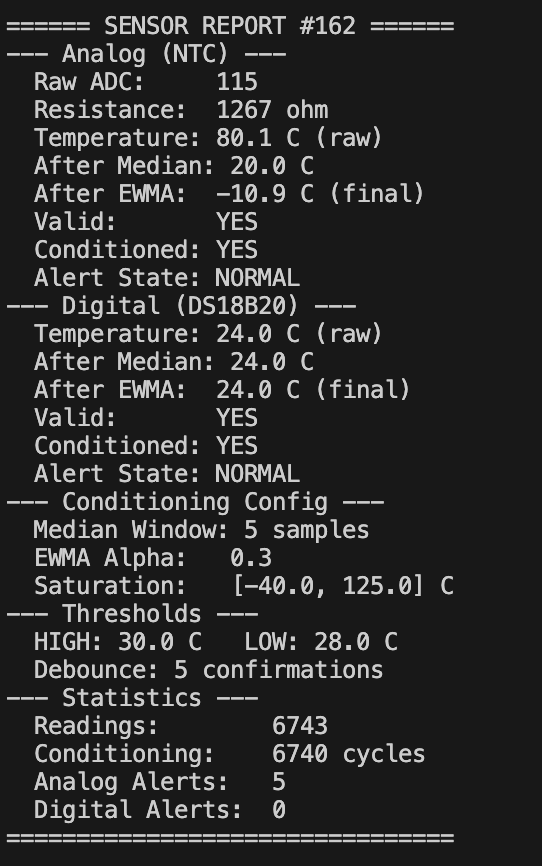
\includegraphics[width=0.85\textwidth]{resources/ObtainedResults/test_spike_rejection.png}%
}{%
    \fbox{\parbox{0.83\textwidth}{\centering\color{gray}\small
        [Screenshot pending --- rapidly change NTC to extreme value then back.\\
        STDIO report showing Raw jumps to $\sim$80\textdegree C while Median and EWMA\\
        remain near 25\textdegree C. Alert state stays NORMAL.\\
        Save to resources/ObtainedResults/test\_spike\_rejection.png]}}%
}
\caption{Spike rejection --- median filter removes impulsive noise while EWMA remains stable}
\label{fig:test_spike}
\end{figure}

The STDIO report captured during this test clearly shows the divergence between the raw and conditioned values. While the raw temperature briefly shows the spike, the median-filtered value remains stable, and the EWMA output tracks the median with only minimal deviation. The alert state remains ``NORMAL'' throughout, demonstrating that the conditioning pipeline successfully shields the threshold detection from transient sensor anomalies.

\subsubsection{Test 3: Signal Smoothing (EWMA Validation)}

To validate the EWMA smoothing behavior, the NTC temperature is gradually increased from 25\textdegree C to 35\textdegree C over several seconds. With an alpha of 0.3, the EWMA responds to changes but smooths the transition, producing a gradual curve rather than following the raw signal step-by-step.

The EWMA update equation $y_n = \alpha \cdot x_n + (1 - \alpha) \cdot y_{n-1}$ means that each new sample contributes only 30\% of the new output, while the previous output contributes 70\%. This results in a first-order exponential approach to the new steady-state value, with a time constant approximately equal to $\tau = T_s / \alpha$ where $T_s$ is the sampling period.

\begin{figure}[H]
\centering
\IfFileExists{resources/ObtainedResults/test_signal_smoothing.png}{%
    \includegraphics[width=0.85\textwidth]{resources/ObtainedResults/test_signal_smoothing.png}%
}{%
    \fbox{\parbox{0.83\textwidth}{\centering\color{gray}\small
        [Screenshot pending --- gradually increase NTC temperature from 25\textdegree C\\
        to 35\textdegree C. STDIO reports showing raw changes faster than EWMA,\\
        with EWMA smoothly tracking toward the new value.\\
        Save to resources/ObtainedResults/test\_signal\_smoothing.png]}}%
}
\caption{Signal smoothing --- EWMA produces gradual transitions during temperature ramp}
\label{fig:test_smoothing}
\end{figure}

The serial output during the ramp-up shows successive STDIO reports where the raw temperature increases in discrete steps (as the slider is moved), the median follows closely (since the change is sustained rather than impulsive), and the EWMA lags behind, producing a smooth exponential approach. This demonstrates the trade-off inherent in EWMA filtering: lower alpha values provide better noise rejection but introduce greater response delay, while higher alpha values track changes faster but provide less smoothing.

\subsubsection{Test 4: Threshold Alert on Conditioned Values}

A key architectural difference between Lab 3.1 and Lab 3.2 is that the ThresholdAlert FSM receives the conditioned EWMA value rather than the raw sensor reading. This test verifies that alert triggering is based on the smoothed output by raising the NTC temperature above 30\textdegree C and observing the alert behavior.

Because the EWMA introduces a delay in tracking the actual temperature, the alert activation occurs later than it would if the raw value were used. The conditioned value must exceed 30\textdegree C for 5 consecutive debounce cycles, and since the EWMA approaches the threshold gradually, the total latency from temperature change to alert activation is longer than in Lab 3.1 but significantly more robust against false triggers.

\begin{figure}[H]
\centering
\IfFileExists{resources/ObtainedResults/test_threshold_alert.png}{%
    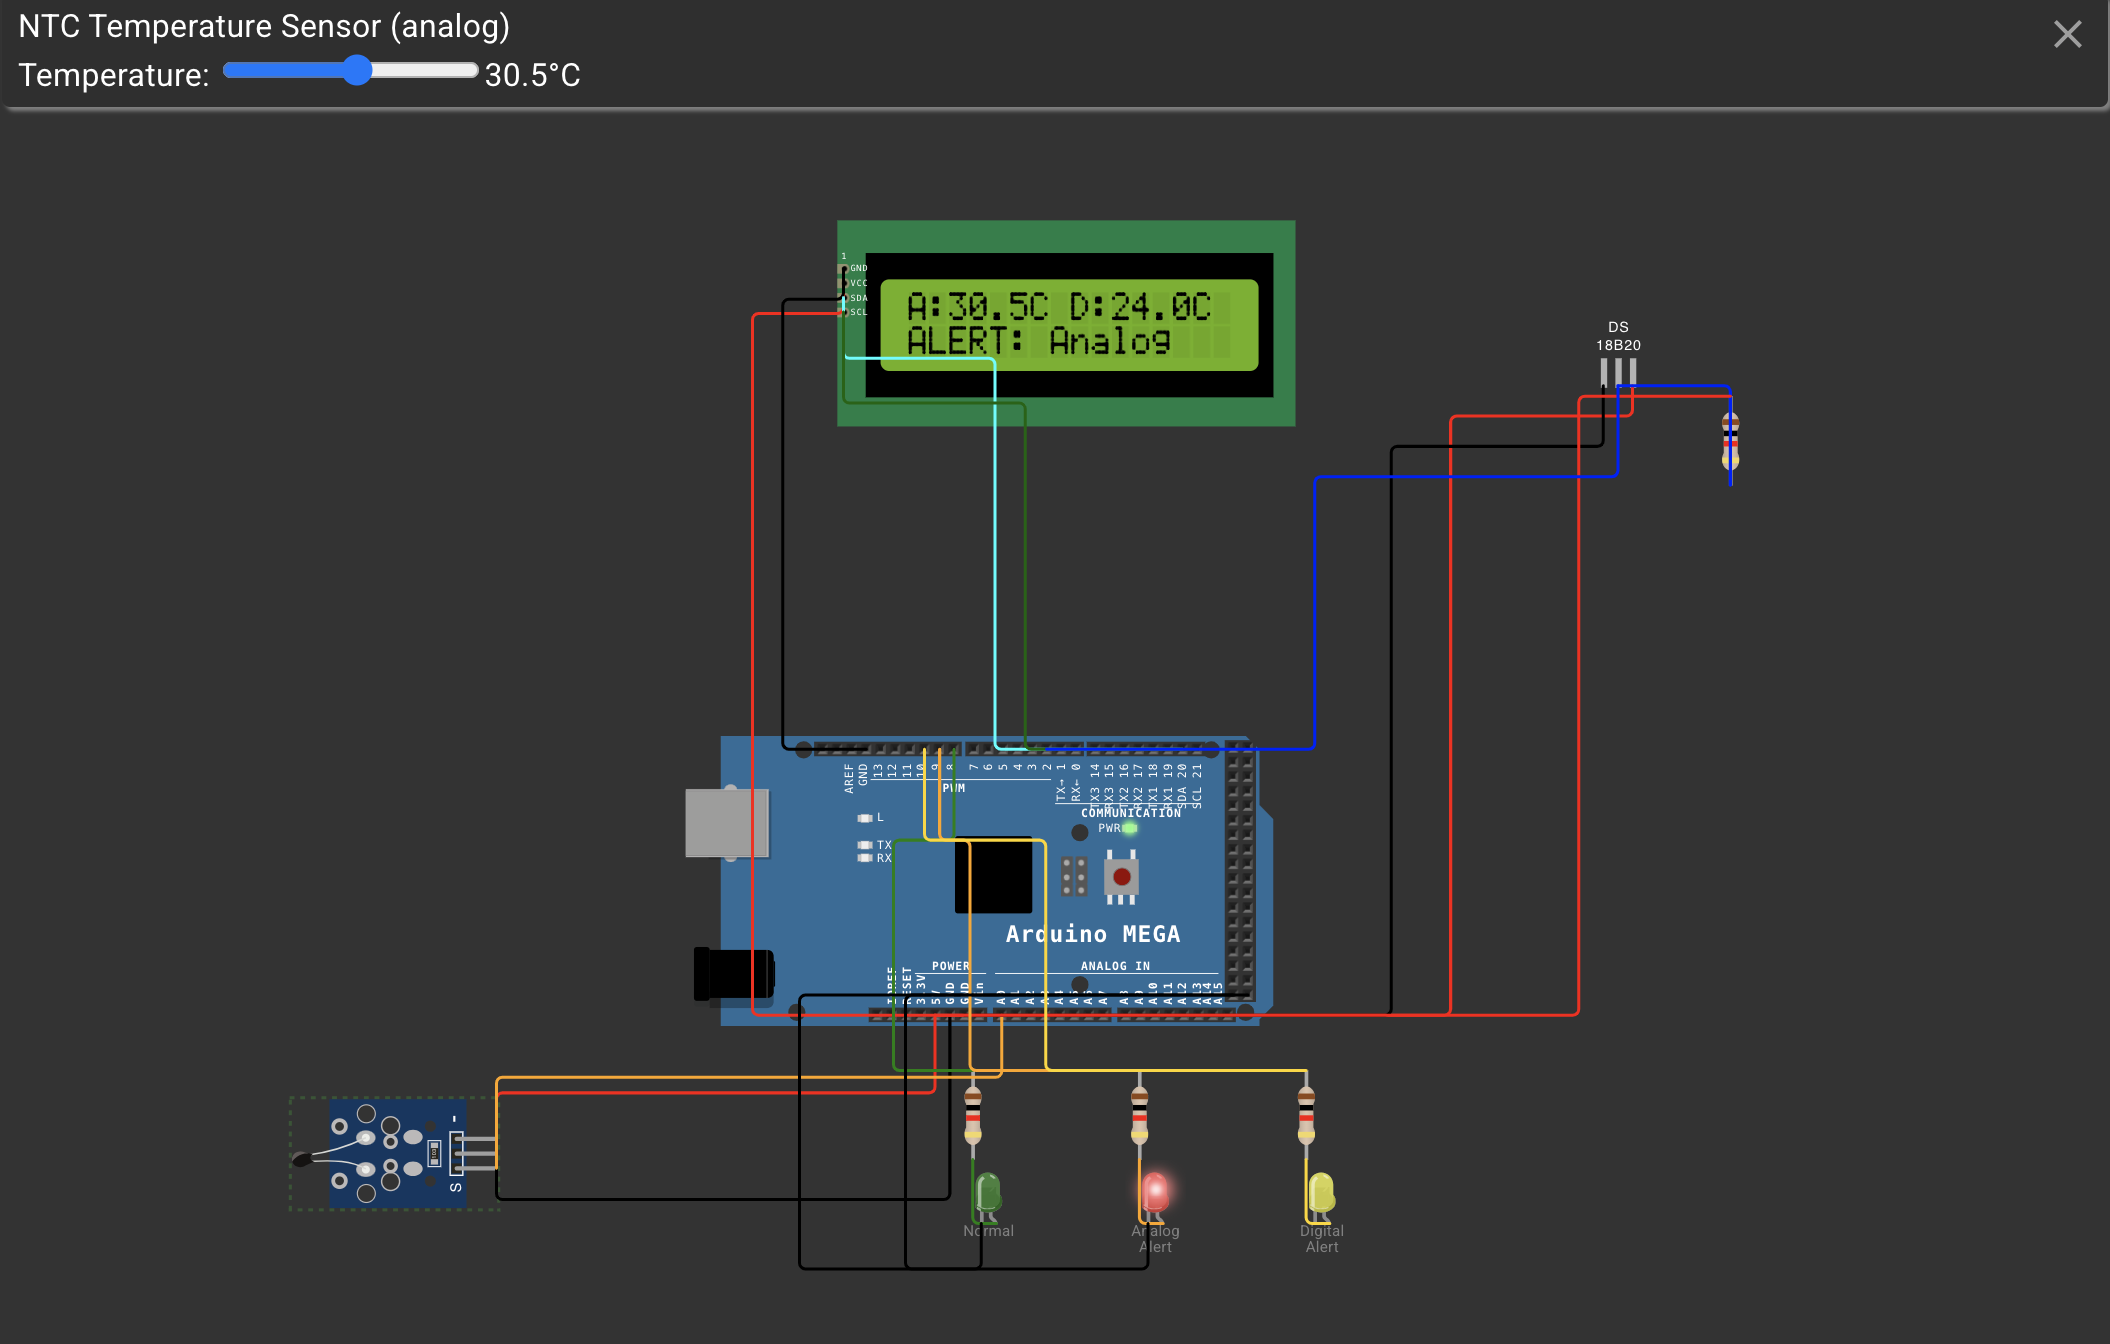
\includegraphics[width=0.85\textwidth]{resources/ObtainedResults/test_threshold_alert.png}%
}{%
    \fbox{\parbox{0.83\textwidth}{\centering\color{gray}\small
        [Screenshot pending --- raise NTC above 30\textdegree C. STDIO shows raw\\
        exceeds threshold before EWMA does. Red LED activates after EWMA\\
        crosses threshold and debounce completes. Green LED turns off.\\
        Save to resources/ObtainedResults/test\_threshold\_alert.png]}}%
}
\caption{Threshold alert on conditioned values --- alert triggers based on EWMA, not raw}
\label{fig:test_threshold}
\end{figure}

The STDIO report confirms the expected behavior: the raw temperature exceeds 30\textdegree C several cycles before the EWMA value crosses the threshold. Once the EWMA exceeds 30\textdegree C, the debounce counter begins incrementing, and after 5 consecutive confirmations, the alert transitions to ALERT\_ACTIVE. The red LED turns on solidly, the green LED turns off, and the LCD status changes from ``System: OK'' to ``ALERT: Analog''. This demonstrates that the conditioning pipeline and threshold detection work together correctly, with the alert reflecting the smoothed system state rather than instantaneous noise.

\subsubsection{Test 5: Saturation Test}

The saturation stage clamps input values to the physically valid range of [$-$40, 125]\textdegree C, corresponding to the NTC thermistor's operating envelope. To validate this behavior, the NTC slider is set to extreme positions that produce ADC readings near the rail voltages, resulting in computed temperatures outside the valid range.

When the computed temperature exceeds 125\textdegree C or falls below $-$40\textdegree C, the saturation stage clamps the value to the nearest bound before it enters the median filter. This prevents physically impossible readings from corrupting the median window and propagating through the EWMA to the alert system.

\begin{figure}[H]
\centering
\IfFileExists{resources/ObtainedResults/test_saturation.png}{%
    \includegraphics[width=0.85\textwidth]{resources/ObtainedResults/test_saturation.png}%
}{%
    \fbox{\parbox{0.83\textwidth}{\centering\color{gray}\small
        [Screenshot pending --- set NTC slider to extreme positions.\\
        STDIO report showing raw temperature outside valid range\\
        while median and EWMA are clamped to [$-$40, 125]\textdegree C.\\
        Save to resources/ObtainedResults/test\_saturation.png]}}%
}
\caption{Saturation test --- values clamped to valid sensor operating range}
\label{fig:test_saturation}
\end{figure}

The STDIO report during the saturation test shows the raw computed temperature at an extreme value while the conditioned output remains within the valid range. The saturation bounds of [$-$40, 125]\textdegree C are displayed in the ``Conditioning Config'' section of the report, confirming that the configured limits are correctly applied. This stage serves as a first line of defense against sensor hardware faults or wiring issues that could produce erratic ADC readings.

\subsection{Periodic Report Output}

The structured STDIO report generated every 2 seconds provides comprehensive diagnostic information that exposes all stages of the conditioning pipeline. Unlike Lab 3.1 which reported only raw temperatures and alert states, the Lab 3.2 report includes separate lines for raw, median-filtered, and EWMA values for each sensor channel, along with the conditioning configuration and pipeline status.

\begin{figure}[H]
\centering
\IfFileExists{resources/ObtainedResults/test_report.png}{%
    
\includegraphics[width=0.85\textwidth]{resources/ObtainedResults/test_report.png}%
}{%
    \fbox{\parbox{0.83\textwidth}{\centering\color{gray}\small
        [Screenshot pending --- capture the serial monitor showing\\
        a full structured STDIO report with all conditioning pipeline\\
        fields visible: raw, median, EWMA for both sensors.\\
        Save to resources/ObtainedResults/test\_report.png]}}%
}
\caption{Structured STDIO diagnostic report with conditioning pipeline values}
\label{fig:test_report}
\end{figure}

The report is organized into five sections:
\begin{itemize}
    \item \textbf{Analog (NTC)}: Raw ADC value, computed resistance, raw temperature, median-filtered temperature, EWMA temperature, validity flag, conditioning status (``YES'' once the window is filled, ``FILLING'' during startup), and alert FSM state with debounce progress.
    \item \textbf{Digital (DS18B20)}: Raw temperature, median-filtered temperature, EWMA temperature, validity flag, conditioning status, and alert FSM state with debounce progress.
    \item \textbf{Conditioning Config}: Median window size (5 samples), EWMA alpha (0.3), and saturation bounds ([$-$40, 125]\textdegree C).
    \item \textbf{Thresholds}: High threshold (30.0\textdegree C), low threshold (28.0\textdegree C), and debounce confirmation count (5).
    \item \textbf{Statistics}: Total acquisition readings, conditioning cycles, and cumulative alert activation counts for both channels.
\end{itemize}

This detailed reporting format enables thorough verification of the conditioning pipeline's behavior at every stage and provides the diagnostic visibility necessary for tuning the filter parameters (window size, alpha) during system development.

\subsection{Verification Summary}

The following table summarizes the test results for all scenarios:

\begin{table}[H]
\centering
\begin{tabular}{|l|c|l|}
\hline
\textbf{Test Scenario} & \textbf{Result} & \textbf{Observation} \\
\hline
Normal operation           & PASS & Raw $\approx$ Median $\approx$ EWMA at steady state \\
Spike rejection            & PASS & Median rejects single-sample outlier \\
Signal smoothing           & PASS & EWMA produces gradual transitions \\
Threshold on conditioned   & PASS & Alert triggers on EWMA, not raw \\
Saturation clamping        & PASS & Values clamped to [$-$40, 125]\textdegree C \\
LCD page alternation       & PASS & Conditioning config displayed on Page 1 \\
STDIO report format        & PASS & All pipeline stages visible \\
\hline
\end{tabular}
\caption{Test verification summary for Lab 3.2}
\label{tab:test_summary}
\end{table}

All test scenarios produced the expected behavior, confirming that the three-stage conditioning pipeline correctly processes raw sensor readings and that the threshold alert system operates on the conditioned output as designed.
